%%=============================================================================
%% Resultaten
%%=============================================================================

\chapter{\IfLanguageName{dutch}{Vergelijking van resultaten}{Comparing results}}
\label{ch:resultaten}

\section{\IfLanguageName{dutch}{Inleiding}{Preface}}
\label{sec:resultaten-inleiding}
Na het uitvoeren van de code zoals besproken in Hoofdstuk \ref{ch:methodologie} werd er een CSV\footnote{https://docs.google.com/spreadsheets/d/1vGC7rQ9PlnfjhAAsU6fJdlmlrZMXW1S3uCMdqmFghqI} gegenereerd. In deze CSV werd er voor iedere afbeelding in de dataset 3 labels opgehaald per API's.

Op basis van deze CSV werd er voor iedere label een score vastgelegd zoals besproken in Sectie~\ref{sec:scoren-van-labels}. Daarnaast werd voor ieder gevonden label aangeduid of de threshold van 75\% zekerheidsgraad gehaald werd, de volledige resultaten van de scoring kunnen teruggevonden worden in deze\footnote{https://docs.google.com/spreadsheets/d/1oCs-aDkhPV2lCayjLyzUPF0SlAUZ7vMjzD4DYuIluyE} Google Sheet. In de sheet kan men ook de aggregatie van de resultaten en grafieken terugvinden.

In de eerste sectie van dit hoofdstuk worden de resultaten besproken waarbij labels met een zekerheidsgraad onder de threshold genegeerd worden. In de volgende sectie worden de resultaten waarbij de zekerheidsgraad onder de treshold ligt besproken en wordt de impact van de threshold per API verder toegelicht. Ten slotte wordt de peformantie van iedere API besproken en wordt er een besluit getrokken in functie van de onderzoeksvraag.

\section{\IfLanguageName{dutch}{Resultaten met thresholding toegepast}{Results with thresholding on confidence}}
\label{sec:resultaten-met-thresholding}
In de genormaliseerde staafdiagram op Figuur~\ref{fig:resultswiththresholding} worden het aantal resultaten per score van iedere computer vision API afgebeeld, waarbij de labels met een zekerheidsgraad onder 75\% werden genegeerd. Figuur~\ref{fig:resultswiththresholdingnotstacked} beeldt dezelfde data af maar in absolute waardes.

De percentages besproken in de volgende subsecties zijn steeds de percentages van het totaal van de respectievelijke scores zoals afgebeeld in Figuur~\ref{fig:resultswiththresholding}.

Het is belangrijk om te vermelden dat bij imagga significant meer resultaten onder de threshold vielen waardoor de samplegroep in deze sectie slechts 31 scores omvat, zie Figuur~\ref{fig:resultsthresholding}.

\begin{figure}
    \centering    
    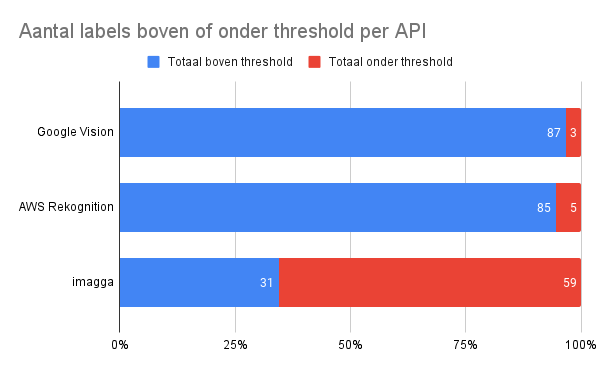
\includegraphics[width=\textwidth]{resultsthresholding}
    \caption{Aantal labels boven of onder de threshold per API}
    \label{fig:resultsthresholding}
\end{figure}

\begin{figure}
    \centering    
    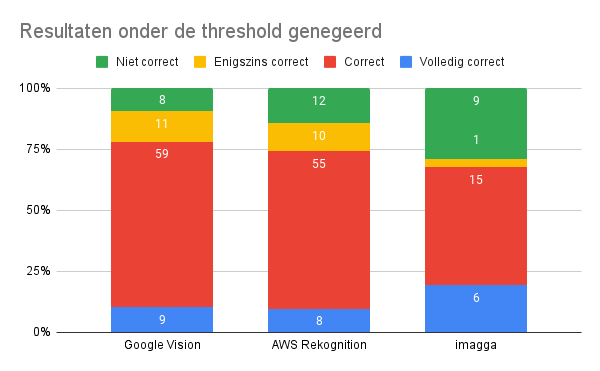
\includegraphics[width=\textwidth]{resultswiththresholding}
    \caption{Genormaliseerde resultaten label-herkenning per API, resultaten onder de threshold genegeerd}
    \label{fig:resultswiththresholding}
\end{figure}

\begin{figure}
    \centering    
    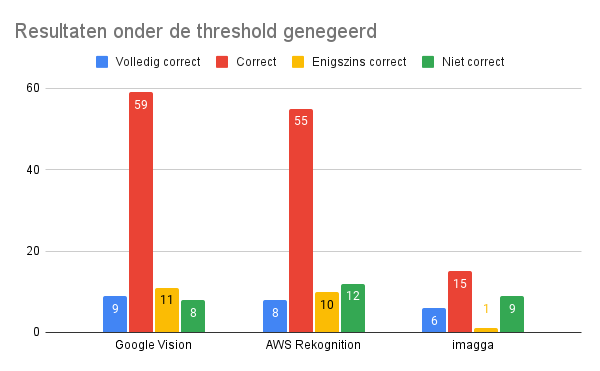
\includegraphics[width=\textwidth]{resultswiththresholdingnotstacked}
    \caption{Resultaten label-herkenning per API, resultaten onder de thresholding genegeerd}
    \label{fig:resultswiththresholdingnotstacked}
\end{figure}

%Bij zowel Google Vision als AWS Rekognition zijn de resultaten gelijkaardig, imagga scoort significant verschillend. Aangezien de resultaten van Google Vision en AWS Rekognition dicht bij elkaar liggen worden deze naast elkaar besproken. 

\subsection{\IfLanguageName{dutch}{Volledig correct}{volledig correct}}
\label{sec:resultaten-volledig-correct}
Percentages in volgorde van grootte:
\begin{itemize}
    \item Imagga: 19,4\%
    \item Google Vision: 10,3\%
    \item AWS Rekognition: 9,4\%
\end{itemize}

imagga behaalt in deze categorie een signifcant hogere score dan Google Vision of AWS Rekognition met een verschil van +-10\%. Google Vision en AWS Rekognition zijn onderling niet significant verschillend.
imagga geeft gemiddeld minder algemene labels terug dan Google Vision of AWS Rekognition, het durft vaker een specifiek object of concept benoemen. Deze manier van labelen zorgt voor een hoger percentage 'volledig correct'.

\subsection{\IfLanguageName{dutch}{Correct}{Correct}}
\label{sec:resultaten-correct}
Percentages in volgorde van grootte:
\begin{itemize}
    \item Google Vision: 67,8\%
    \item AWS Rekogniion: 64,7\%
    \item imagga: 48,4\%
\end{itemize}

Opnieuw scoren Google Vision en AWS Rekognition niet significant verschillend van elkaar, er is echter een kloof van 15\% tot 19\% naar imagga. Uit deze data kan gesteld worden dat Google Vision en AWS Rekognition sterk zijn in labels vinden die correct zijn, maar eerder in de algemene vorm. Bij Google Vision viel in de resultaten op dat er vaak het label 'sky' werd geretourneerd en bij AWS Rekognition 'Person'. Deze objecten zijn meestal niet de belangrijkste maar zijn wel 'correct'.

\subsection{\IfLanguageName{dutch}{Enigszins correct}{Somewhat correct}}
\label{sec:resultaten-enigszins-correct}
Percentages in volgorde van grootte:
\begin{itemize}
    \item Google Vision: 12,6\%
    \item AWS Rekogniion: 11,8\%
    \item imagga: 3,2\%
\end{itemize}

Google Vision en AWS Rekognition zijn net zoals bij de voorgaande categorieën niet significant verschillend. imagga scoort ook in deze categorie een stuk lager in vergelijking met de andere twee API's. Zoals in de vorige sectie besproken geven zowel Google Vision als AWS Rekognition regelmatig labels terug die algemeen zijn in plaats van specifiek. Labels in de categorie 'enigszins correct' geven een te vage beschrijving om waarde toe te voegen aan de afbeelding. Zo geeft AWS Rekognition bij sample12 - een foto van fruit op de markt - de label 'plant' terug. imagga geeft gemiddeld meer specifieke labels terug, wat de lage score in deze categorie verklaart.

\subsection{\IfLanguageName{dutch}{Niet correct}{niet correct}}
\label{sec:resultaten-niet-correct}
Percentages in oplopende volgorde van grootte:
\begin{itemize}
    \item Google Vision: 9,2\%
    \item AWS Rekogniion: 14,1\%
    \item imagga: 29\%
\end{itemize}

In deze categorie valt er een verschil op te merken van 4,9\% tussen Google Vision en AWS Rekognition. Dit verschil kan als niet significant beschoud worden maar kan op een trend wijzen waarbij Google Vision minder foute resultaten retourneert dan AWS Rekognition. imagga scoort in deze categorie relatief slecht, er zijn significant meer foute resultaten als bij Google Vision of AWS Rekognition. Opnieuw kunnen deze verschillen verklaard worden door de tendens van imagga om meer specifieke labels terug te geven, dit zorgt voor meer 'volledig correct' maar de keerzijde is dat er ook meer 'niet correct' labels zijn. Google Vision en AWS Rekognition spelen het eerder veilig om zo de foutmarges zo laag mogelijk te houden.

\section{\IfLanguageName{dutch}{Resultaten met thresholding niet toegepast}{Results without thresholding}}
\label{sec:resultaten-zonder-thresholding}
In Figuur~\ref{fig:resultswithoutthresholding} worden de opgetelde scores per API genormaliseerd afgebeeld, de scores onder de threshold werden in deze grafiek niet genegeerd.

Het verschil in percentages tussen thresholding genegeerd en niet genegeerd zijn niet significant voor zowel Google Vision als AWS Rekognition. Dit kan verklaard worden doordat beide respectievelijk slechts 3 en 5 labels onder de threshold hadden.

Bij imagga worden er wel significante verschillen opgemerkt, er zijn 27 meer 'correct' labels en 26 meer 'niet correct' labels. Procentueel gezien krijgen we volgende wijzigingen:
\begin{itemize}
    \item Volledig correct: 7,8\% (-11,6\%)
    \item Correct: 46,7\% (-1,7\%) 
    \item Enigszins correct: 6,7\% (+3,5\%)
    \item Niet correct: 38,9\% (+9,9\%)
\end{itemize}

Er kan gesteld worden dat imagga veruit het meest terughoudend is met de zekerheidgraad wat er voor zorgt dat er veel meer labels onder de threshold vallen. Dit lijkt een correct manier van labelen voor imagga aangezien het accepteren van een lagere zekerheidsgraad procentueel gezien tot meer verkeerde resultaten leidt. Verder viel bij het analyseren van de resultaten op dat imagga de enige API is die zekerheidsgraden van 100\% terug geeft, opnieuw kan men stellen dat imagga ofwel heel correct is, ofwel heel incorrect is.

\begin{figure}
    \centering    
    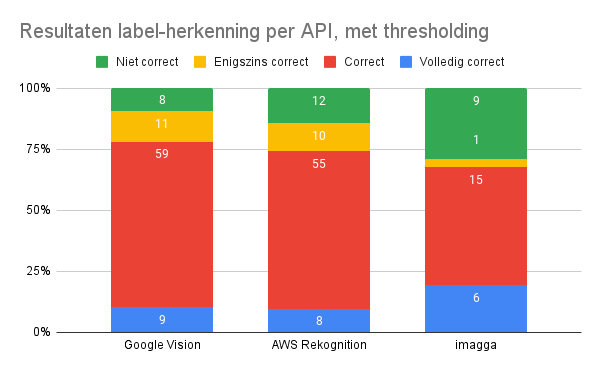
\includegraphics[width=\textwidth]{resultswithoutthresholding}
    \caption{Resultaten label-herkenning per API, zonder thresholding}
    \label{fig:resultswithoutthresholding}
\end{figure}

\section{\IfLanguageName{dutch}{Snelheid per API}{Speed per api}}
\label{sec:snelheid-per-api}
Alhoewel snelheid van verwerking geen belangrijk doel is in de onderzoeksvraag van deze Bachelorproef wordt ze toch kort geanalyseerd als bijkomstige informatie.

Van iedere call werd bijgehouden hoe snel labels geretourneerd werden, deze data werd verwerkt tot gemiddeldes:
\begin{itemize}
    \item Google Vision: 594,17 milliseconden per call
    \item AWS Rekognition: 1068,59 milliseconden per call
    \item Imagga: 1641,42 milliseconden per call
\end{itemize}

imagga heeft de traagste verwerking, dit wordt beïnvloed door de vereiste  dat afbeeldingen altijd eerst moeten geupload worden voor ze kunnen gelabeld worden, er moeten 2 calls gemaakt worden in plaats van 1 call voor Google Vision of AWS Rekognition.

Er kan gesteld worden dat automatische labeling gemiddeld sneller verloopt dan manuele labeling; Archief Gent schat in dat 10.000 milliseconden een absoluut minimum is om 3 labels toe te wijzen aan een afbeelding.

\section{\IfLanguageName{dutch}{Resultaten in functie van de onderzoeksvraag}{Resolution}}
\label{sec:besluit}
Op basis van de data besproken in vorige secties kan samengevat worden dat de resultaten voor Google Vision en AWS Rekognition onderling weinig verschillend zijn. imagga daarintegen verschilt doordat het meer specifieke labels teruggeeft maar ook doordat het een lagere zekerheidgraad heeft voor de gevonden labels.

De doelstellingen uitgedrukt in de probleemstelling worden in deze sectie besproken aan de hand van de resultaten van het onderzoek.

\subsection{\IfLanguageName{dutch}{Foto's zoekbaar maken door middel van AI}{Make pictures searchable with AI}}
\label{sec:resultaten-doelstelling1}
Zowel Google Vision, AWS Rekognition als imagga zijn in staat om foto's zoekbaar te maken op basis van AI.

\subsection{\IfLanguageName{dutch}{De oplossing moet gemakkelijk te gebruiken zijn}{Ease of use}}
\label{sec:resultaten-doelstelling2}
De API's besproken in dit onderzoek zijn allen gemakkelijk te gebruiken voor een persoon met een basiskennis aan IT. Er kan gesteld worden dat een gemiddeld bedrijf de kennis in huis heeft, of de kennis kan huren, om integratie met een computer vision API op te zetten.

\subsection{\IfLanguageName{dutch}{De oplossing moet breed bruikbaar zijn; voor veel verschillende soorten foto-archieven}{Solution must be usable for many different types of pictures}}
\label{sec:resultaten-doelstelling3}
In de testdata gebruikt in dit onderzoek werden er verschillende soorten afbeeldingen aangeboden: landschappen; evenementen; gebouwen; postkaarten; zwart-wit fotos; mensen; interieur. De API's konden bij alle soorten foto's labels toewijzen.

\subsection{\IfLanguageName{dutch}{Foutmarge van maximaal 15\%}{Margin of error not higher than 15\%}}
\label{sec:resultaten-doelstelling4}
Enkel Google Vision (9,2\%) en AWS Rekognition (14,1\%) behalen deze doelstelling, imagga haalt een foutmarge van 29\%. 

\section{\IfLanguageName{dutch}{Besluit}{Resolution}}
\label{sec:resultaten-besluit}
Uit vorige secties werd duidelijk dat zowel AWS Rekognition en Google Vision beide de vooropgezette doelstellingen halen. Beiden API's scoren op de meeste vlakken gelijkaardig, Google Vision haalt niet-significant betere scores. Er moet meer onderzoek met grotere datasets worden uitgevoerd om deze trend al dan niet verder te bevestigen.

imagga behaalt enkel de doelstelling rond foutmarge niet en voldoet bijgevolg niet aan de business case.

Na het uitvoeren van het onderzoek werd het duidelijk dat een belangrijk onderdeel van de configuratie zich bevindt in de threshold van de zekerheidsgraad. Een te lage threshold zorgt voor false positives terwijl een te hoge threshold zorgt voor false negatives. imagga gaf slechts bij 65,6\% van de labels een zekerheidsgraad boven de threshold, de threshold zou verlaagd kunnen worden maar in sectie \ref{sec:resultaten-zonder-thresholding} wordt duidelijk dat dit leidt tot een significante daling in kwaliteit van de labels. In een productie-situatie is het niet haalbaar dat er gemiddeld slechts 1 label per afbeelding wordt toegewezen, dit is een extra reden waarom imagga, in zijn huidige vorm, niet bruikbaar is voor de business-case van deze Bachelorproef. 

Verder valt het op dat Google Vision en AWS Rekognition laag (+- 10\%) scoren voor de categorie 'volledig correct'. Deze scores worden eenerzijds beïnvloed door de kwaliteit van de labels in de dataset maar anderzijds valt het op dat beide API's geen labels teruggeven die gedetailleerd genoeg zijn. Verder ontbreekt het de API's aan context waardoor ze sommige labels onmogelijk kunnen voorspellen. 
Zo kon geen van de API's voorspellen dat sample17 (een foto van vuurwerk) de label 'nieuwjaar' had in de Beeldbank.  Enkel de persoon die de foto gemaakt heeft kan aan de hand van de context dit label aanvullen.

Een tweede voorbeeld waarbij het gebrek aan context de API's parten speelt is het label 'vintage clothing' dat Google Vision toewees aan sample28. sample28 is een foto van een militaire muziekkapel uit 1916 - de kledij die de mensen op de foto dragen wordt vandaag inderdaad als vintage aangeduid maar toch is de label incorrect in de context van de foto.